\documentclass{beamer}

\usepackage[utf8]{inputenc}
\usepackage[spanish]{babel}
\usepackage{fontenc}

\usepackage{pgfpages}
\setbeameroption{show notes on second screen=right} % Notas + diapositivas

\usepackage{graphicx}

\title{Presentaciones en \LaTeX}
\author{Ondiz}
\institute{Home, sweet home}
\date{\today}

\usetheme{Bergen}
\usefonttheme{serif}
\usecolortheme{rose}

% Título de la presentación en negrita
\setbeamerfont{title}{series=\bfseries}

% Todos los títulos en rosa con el fondo blanco
\setbeamercolor{title}{fg=magenta, bg=white}
\setbeamercolor{titlelike}{fg=magenta, bg=white}

% Sin símbolos de navegación
\setbeamertemplate{navigation symbols}{}

% Flechas para indicar ítems en listas 
\setbeamertemplate{itemize item}{$\Rightarrow$}

% Diapositiva con el título de sección al iniciar sección
\AtBeginSection{
  \begin{frame}
  \vfill
  % Caja con colores de título
  \begin{beamercolorbox}[center]{title}
    \usebeamerfont{title} % Fuente de título
    \insertsectionhead % Nombre de sección
  \end{beamercolorbox}
  \vfill
  \end{frame}
}


% Índice mostrando subsección actual al iniciar subsección
\AtBeginSubsection
{   \begin{frame}{Índice}
        \tableofcontents[currentsection,
        currentsubsection,
        sectionstyle=show/hide,
        subsectionstyle=show/shaded/hide] 
    \end{frame}
}

% Índice en la diapositiva

\def\insertauthorindicator{}% Default is "Who?"
\def\insertinstituteindicator{}% Default is "From?"
\def\insertdateindicator{}% Default is "When?"

\usepackage{media9}
\usepackage{multimedia}

\usepackage{hyperref}

\begin{document}
 
 \begin{frame}
  \maketitle
  \note{Notas}
 \end{frame}
 
 \begin{frame}{Índice}
  \tableofcontents
  \note{Más notas}
 \end{frame}
 
 \section{Introducción}
 \subsection{Primera parte}

 \begin{frame}{Introducción}
  \begin{itemize}[<+->]
   \item Ítem 1
   \item Ítem 2
  \end{itemize}
  \note<1>{Notas para el ítem 1}
  \note<2>{Notas para el ítem 2}
 \end{frame}
 
 \subsection{Segunda parte}
 
   \begin{frame}{Introducción}
     \begin{block}{Vídeos}
      % Vídeo con multimedia
      \movie{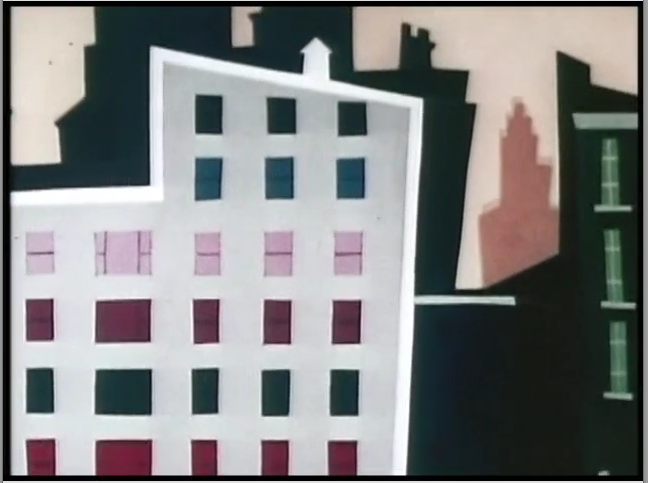
\includegraphics[width=0.45\textwidth]{poster}}{popeye.mp4}
      % Vídeo con media9
      \includemedia{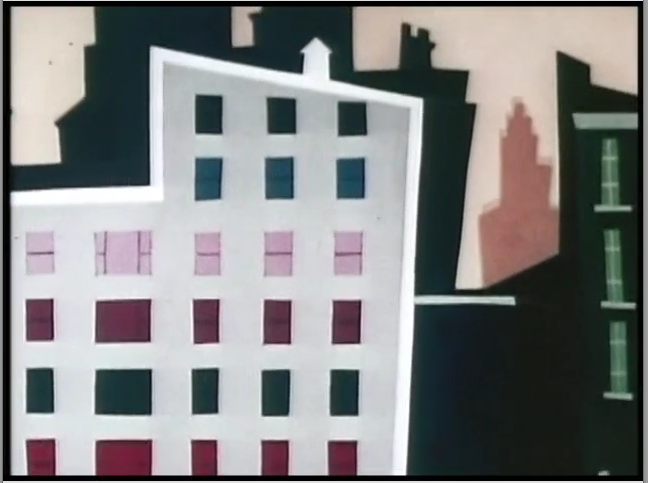
\includegraphics[width=0.45\textwidth]{poster}}{popeye.mp4}
      
      % Vídeo con href
      \href{run:popeye.mp4}{Vídeo}
     \end{block}

   \end{frame}
 
\end{document}
